%!TEX root = ../thesis.tex

%jama -- macro-micro integration architecture chapter

\chapter{Macro--Micro Integration Architecture}
\label{ch:integration}

\section{Overview}
\label{sec:integration_overview}

%jama
The present chapter describes how the macro-level MPC framework and the micro-level agent-based model are connected into a coherent two-level simulation system.
The integration is designed to be minimal and unidirectional: the macro model generates time-varying transmission rate signals $\beta_1(t)$ and $\beta_2(t)$, and these signals are passed directly to the agent-based model as inputs.
No state information flows back from the ABM to the MPC controller.

Figure~\ref{fig:block_diagram} shows the overall system architecture.

\begin{figure}[ht]
  \centering
  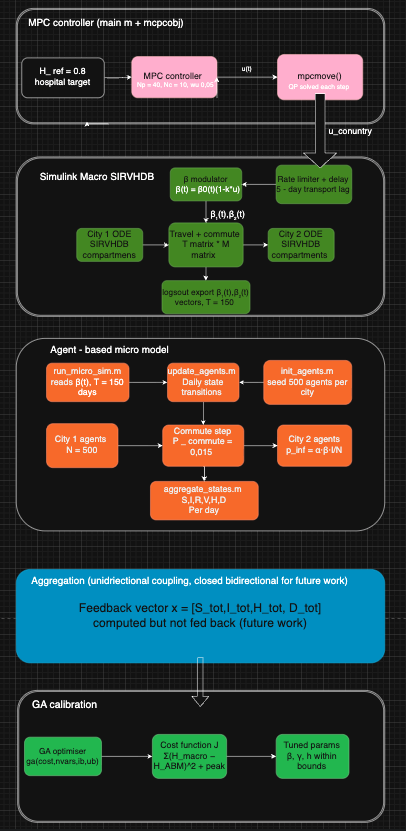
\includegraphics[width=0.90\textwidth]{Figures/jama/block_diagram_uploaded}
  \caption{%jama
    Overall system architecture connecting the MPC controller,
    the Simulink SIRVHDB macro model, and the agent-based micro model.
    The $\beta(t)$ signals are the sole coupling variable between model levels.}
  \label{fig:block_diagram}
\end{figure}

\section{Interface: $\beta(t)$ Signal Extraction}
\label{sec:beta_interface}

%jama
The Simulink model is run via the \texttt{sim()} function in MATLAB, producing a logged output structure (\texttt{logsout}) containing the time-series signals \texttt{beta\_t1} and \texttt{beta\_t2}.
These signals represent the effective, MPC-modulated transmission rates in City~1 and City~2 respectively, at daily resolution over the simulation horizon ($T = 150$~days).

The \texttt{main.m} script extracts these signals and passes them directly as input to the micro-model simulation function:
\begin{verbatim}
  run_micro_sim(beta_t1_series, beta_t2_series)
\end{verbatim}
This constitutes the complete interface between the macro and micro model levels.
The interface is intentionally minimal: the only data crossing from macro to micro is the pair of length-$T$ column vectors \texttt{beta\_t1\_series} and \texttt{beta\_t2\_series}.
This design choice reflects the unidirectional coupling of the current framework and makes the micro model independent of the macro model's internal state.

\section{Overall Execution Flow}
\label{sec:exec_flow}

%jama
The integration between model levels is managed by \texttt{main.m}.
The overall execution flow proceeds as follows:
\begin{enumerate}
  \item Macro model parameters are loaded from \texttt{SIRVDB\_model\_parameters.m}.
  \item The Simulink model \texttt{SIRVHDB\_MPC\_model} is run via \texttt{sim()} over a 150-day horizon.
  \item The MPC-generated transmission rate time series $\beta_1(t)$ and $\beta_2(t)$ are extracted from the logged signal outputs.
  \item These series are passed to \texttt{run\_micro\_sim()}, which executes the agent-based simulation.
  \item Results from both model levels are plotted and saved.
\end{enumerate}

\section{Parameter Consistency}
\label{sec:param_consistency}

%jama
Ensuring that the macro and micro models operate in a consistent epidemiological regime requires matching of key parameters.
The disease progression rates ($\gamma$, $\gamma_v$, $\gamma_h$, $\mu$, $\mu_v$, $\mu_h$, $h$, $h_v$, $\omega_V$, $\omega_R$) and the breakthrough factor $\eta$ are shared between the two models.
The macro model population is normalised to a fraction of $N_c$ (with $N_c = 500$ in the micro model), so compartment counts in the micro model and fractions in the macro model are directly proportional.

The transmission rate $\beta(t)$ serves as the single coupling variable.
In the macro ODE, $\beta$ appears in the force-of-infection term $\beta \cdot S \cdot I / N$.
In the micro ABM, $\beta$ is used to compute per-contact infection probabilities, scaled by the contact intensity parameter $\alpha = 0.35$ and the proximity factor.
The calibration of $\alpha$ is chosen so that the aggregate ABM infection rate approximately matches the ODE dynamics under the same $\beta$ value.

Table~\ref{tab:shared_params} summarises the parameters shared across both model levels.

\begin{table}[ht]
\centering
\caption{Parameters shared between the macro ODE model and the micro ABM.}
\label{tab:shared_params}
\begin{tabular}{@{}lll@{}}
\toprule
\textbf{Parameter} & \textbf{Description} & \textbf{Value} \\
\midrule
$\beta_{c,\mathrm{nom}}$ & Nominal transmission rate & 0.45 day$^{-1}$ \\
$\gamma$    & Recovery rate, unvaccinated  & $1/12$ day$^{-1}$ \\
$\gamma_v$  & Recovery rate, vaccinated    & $1/9$ day$^{-1}$ \\
$\gamma_h$  & Hospital discharge rate      & $1/25$ day$^{-1}$ \\
$h$         & Hospitalisation rate         & 0.05 \\
$h_v$       & Hospitalisation rate, vaccinated & 0.02 \\
$\mu$       & Fatality rate                & 0.001 day$^{-1}$ \\
$\mu_v$     & Fatality rate, vaccinated    & 0.0005 day$^{-1}$ \\
$\mu_h$     & Fatality rate, hospitalised  & 0.02 day$^{-1}$ \\
$\eta$      & Breakthrough factor          & 0.60 \\
$\omega_R$  & Waning immunity, recovered   & $1/110$ day$^{-1}$ \\
$\omega_V$  & Waning immunity, vaccinated  & $1/140$ day$^{-1}$ \\
\bottomrule
\end{tabular}
\end{table}

\section{Unidirectional vs.\ Bidirectional Coupling}
\label{sec:coupling}

%jama
The current implementation uses unidirectional coupling: the macro model generates $\beta(t)$ independent of the micro model's state, and the micro model consumes this signal without feeding back to the MPC controller.
This design is appropriate for a validation study --- it tests whether the MPC signal is effective in the micro domain without requiring online integration of a stochastic simulator into the MPC feedback loop.

A fully bidirectional coupled system, where the MPC observes aggregated micro-model outputs (e.g., empirical hospital load) and reacts to them, would represent a more realistic and more complex architecture.
Such a system would need to address:
\begin{itemize}
  \item the stochastic nature of micro-model outputs, which would introduce noise into the MPC feedback signal;
  \item the computational cost of running the ABM online within the MPC loop at each sample step;
  \item potential instabilities introduced by stochastic feedback into a controller designed for deterministic plant dynamics.
\end{itemize}
These challenges are recognised as important directions for future work (see Section~\ref{sec:future}).
